\documentclass[border=10pt]{standalone}
\usepackage[svgnames]{xcolor}
\usepackage{amsmath}
\usepackage{pgfplots}
\pgfplotsset{compat=newest}
\usepackage[sfdefault]{FiraSans}
\usepackage{FiraMono}
\renewcommand*\familydefault{\sfdefault}
\begin{document}
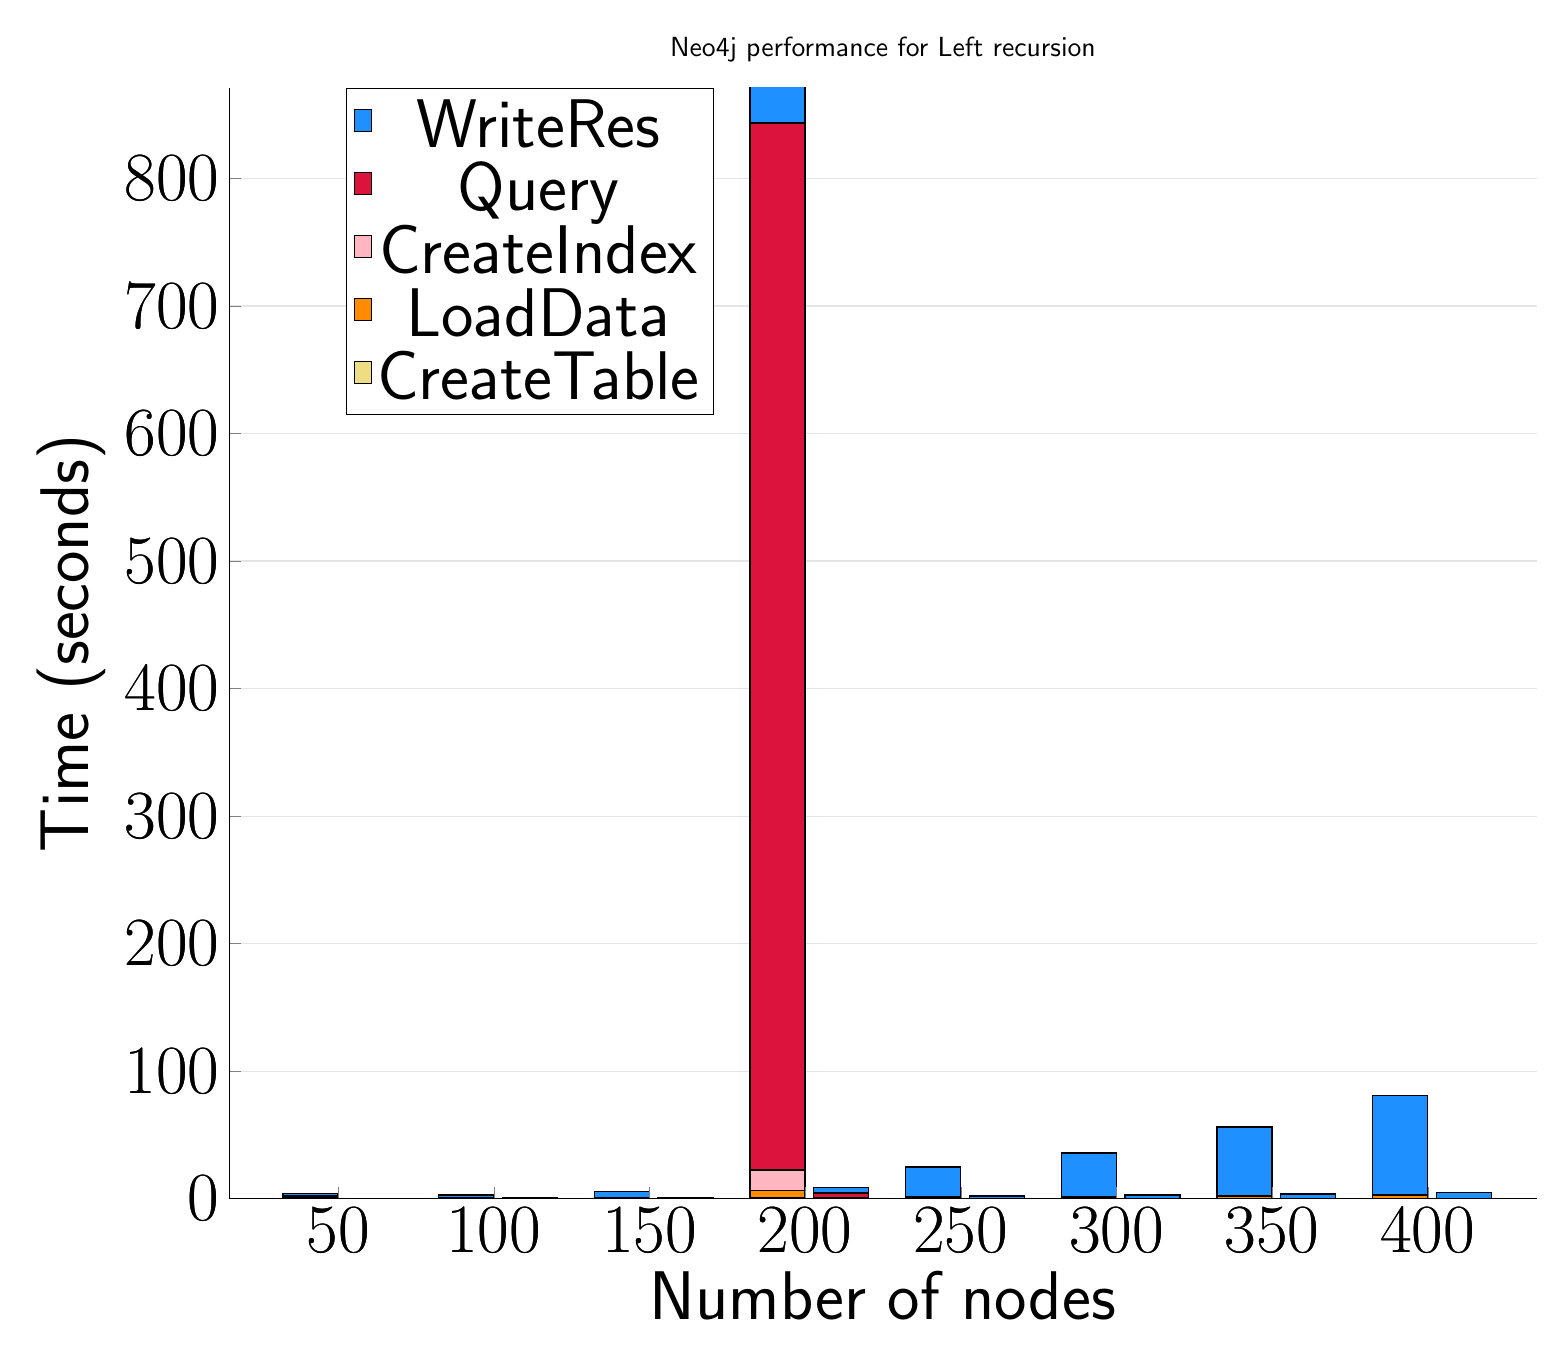
\begin{tikzpicture}
\begin{axis}[
   ybar stacked,
   title={Neo4j performance for Left recursion},
   bar shift=-10pt,
   width=1.5\textwidth,
   bar width=0.7cm,
   ymajorgrids, tick align=inside,
   major grid style={draw=gray!20},
   xtick=data,
   ymin=0, ymax=871.1066666692495,
   axis x line*=bottom,
   axis y line*=left,
   enlarge x limits=0.1,
   legend style={
       at={(0.23, 1)},
       anchor=north,
       legend columns=1,
       font=\Huge,
   },
   ylabel={Time (seconds)},
   xlabel={Number of nodes},
   label style={font=\Huge},
   tick label style={font=\Huge},
]
\addlegendimage{fill=DodgerBlue, draw=black, line width=0.2pt}
\addlegendentry{WriteRes}
\addlegendimage{fill=Crimson, draw=black, line width=0.2pt}
\addlegendentry{Query}
\addlegendimage{fill=LightPink, draw=black, line width=0.2pt}
\addlegendentry{CreateIndex}
\addlegendimage{fill=DarkOrange, draw=black, line width=0.2pt}
\addlegendentry{LoadData}
\addlegendimage{fill=LightGoldenrod, draw=black, line width=0.2pt}
\addlegendentry{CreateTable}
\addplot +[fill=LightGoldenrod, draw=black, line width=0.5pt] coordinates {
    (50, 0.9699999988079071)
    (100, 0.0733333354194959)
    (150, 0.03999999910593033)
    (200, 0.6933333327372869)
    (250, 0.11999999980131786)
    (300, 0.13000000019868216)
    (350, 0.14999999850988388)
    (400, 0.22000000129143396)
};
\addplot +[fill=DarkOrange, draw=black, line width=0.5pt] coordinates {
    (50, 0.586666668454806)
    (100, 0.2633333330353101)
    (150, 0.2800000011920929)
    (200, 5.883333332836628)
    (250, 1.0366666664679844)
    (300, 1.2033333331346512)
    (350, 1.5599999999006589)
    (400, 2.046666666865349)
};
\addplot +[fill=LightPink, draw=black, line width=0.5pt] coordinates {
    (50, 0.09999999900658925)
    (100, 0.19000000009934107)
    (150, 0.14666666835546494)
    (200, 15.74333333472411)
    (250, 0.3999999985098839)
    (300, 0.4466666678587595)
    (350, 0.6233333349227905)
    (400, 0.676666667064031)
};
\addplot +[fill=Crimson, draw=black, line width=0.5pt] coordinates {
    (50, 0.5166666681567827)
    (100, 0.03666666895151138)
    (150, 0.0)
    (200, 821.1066666692495)
    (250, 0.0066666702429453535)
    (300, 0.006666665275891622)
    (350, 0.05999999990065893)
    (400, 0.003333332637945811)
};
\addplot +[fill=DodgerBlue, draw=black, line width=0.5pt] coordinates {
    (50, 1.896666665871938)
    (100, 2.1866666649778685)
    (150, 5.256666665275891)
    (200, 107.20333333065112)
    (250, 23.17666666706403)
    (300, 33.85333333412806)
    (350, 53.8433333337307)
    (400, 77.73333333184321)
};
\end{axis}
\begin{axis}[
   ybar stacked,
   bar shift=13pt,
   width=1.5\textwidth,
   bar width=0.7cm,
   ymajorgrids, tick align=inside,
   major grid style={draw=none},
   xtick=data,
   ymin=0, ymax=871.1066666692495,
   axis x line*=none,
   axis y line*=none,
   enlarge x limits=0.1,
   label style={font=\Huge},
   tick label style={font=\Huge},
]
\addplot +[fill=LightGoldenrod, draw=black, line width=0.5pt] coordinates {
    (50, 0.006666666666666636)
    (100, 0.01666666666666668)
    (150, 0.0033333333333333322)
    (200, 0.013333333333333308)
    (250, 0.006666666666666672)
    (300, 0.0)
    (350, 0.006666666666666657)
    (400, 0.006666666666666672)
};
\addplot +[fill=DarkOrange, draw=black, line width=0.5pt] coordinates {
    (50, 0.006666666666666672)
    (100, 0.0)
    (150, 0.0)
    (200, 0.006666666666666672)
    (250, 0.0)
    (300, 0.0)
    (350, 0.0)
    (400, 0.003333333333333337)
};
\addplot +[fill=LightPink, draw=black, line width=0.5pt] coordinates {
    (50, 0.003333333333333336)
    (100, 0.0)
    (150, 0.010000000000000004)
    (200, 0.5266666666666666)
    (250, 0.003333333333333337)
    (300, 0.01333333333333334)
    (350, 0.006666666666666656)
    (400, 0.0)
};
\addplot +[fill=Crimson, draw=black, line width=0.5pt] coordinates {
    (50, 0.0)
    (100, 0.003333333333333337)
    (150, 0.0)
    (200, 3.9133333333333336)
    (250, 0.003333333333333337)
    (300, 0.0)
    (350, 0.0)
    (400, 0.0)
};
\addplot +[fill=DodgerBlue, draw=black, line width=0.5pt] coordinates {
    (50, 0.12666666666666668)
    (100, 0.4133333333333333)
    (150, 0.7800000000000001)
    (200, 4.090000000000001)
    (250, 2.1)
    (300, 2.7133333333333334)
    (350, 3.716666666666667)
    (400, 4.89)
};
\end{axis}
\end{tikzpicture}

\end{document}
